\documentclass[9pt]{beamer}

% % % % % % % % % %%% Dichiarazione dei pacchetti standard.
\usepackage[italian]{babel}
\usepackage[T1]{fontenc} 
\usepackage[utf8]{inputenc}
\usepackage{amsfonts,amsmath,amssymb}
\usepackage{fancyvrb}
\usepackage{xcolor}
\usepackage[none]{hyphenat}
\usepackage{fancyhdr}
\usepackage{graphicx}
\usepackage{float}
\usepackage{smartdiagram}
\usepackage{subfigure}
\usepackage{tikz}


\definecolor{mygreen}{rgb}{.125,.5,.25}
\definecolor{bleudefrance}{rgb}{0.19, 0.55, 0.91}
%%% Personalizzazione del layout---articolata su cinque livelli.
%\usetheme{Madrid}        % layout complessivo.
%\usetheme{boxes}
%\usetheme{Pittsburgh}
%\usetheme{Median}
%\usetheme{Rochester}
%\usetheme{Pittsburgh}
%\usetheme{Madrid}        % layout complessivo.
%\definecolor{mygreen}{rgb}{.125,.5,.25}
%\definecolor{bleudefrance}{rgb}{0.19, 0.55, 0.91}
%\definecolor{ceruleanblue}{rgb}{0.16, 0.32, 0.75}
%\definecolor{bondiblue}{rgb}{0.0, 0.58, 0.71}
\usetheme{Median}
% \usetheme{Casalbo}
%\usecolortheme[named=ceruleanblue]{structure}
%\useinnertheme{circles} % layout interno. (circles rectangles rounded inmargin)
%\useoutertheme{smoothbars}  % layout esterno. (infolines miniframes smoothbars sidebar
%\usecolortheme{crane} % schema di colori.
%\usefonttheme{structurebold}  %schema dei font.
%\setbeamercovered{dynamic}
%\usecolortheme[named=blue]{structure}
%\usecolortheme{seahorse}
%\useinnertheme{circles} % layout interno. (circles rectangles rounded inmargin)
%\useoutertheme{sidebar}  % layout esterno. (infolines miniframes smoothbars sidebar
%\usecolortheme{crane} % schema di colori.
%\usefonttheme{structurebold}  % schema dei font.
%\usefonttheme{professionalfonts}
%\setbeamercovered{dynamic}
% Inutile dire che se volete tutti i default, potete risparmiarvi gli ultimi
% quattro comandi. 
\theoremstyle{definition}
\newtheorem{definizione}{Definizione}


\newcommand*\tick{\item[\checkmark]}
\newcommand*\fail{\item[\XSolidBrush]}
\renewcommand{\vec}{\boldsymbol}

%%% Titolo e autore.
\title{\textbf{Modellazione di un reattore nucleare LFR e implementazione
su piattaforma con accoppiamento neutronico-termoidraulico}}
%\subtitle{?}
\author{Marco Lanconelli}
% \institute{University of Bologna, DIN, Lab. of Montecuccolino, Italy}
% \date{\tt Technical Meeting on the Benefits and Challenges of Fast Reactors of the SMR Type, 26 September 2019}


\begin{document}


\begin{frame}
  \titlepage
\end{frame}

% \begin{frame}
%  \frametitle{Indice}
%  \tableofcontents
% \end{frame}



\section{Introduzione}

% \begin{frame}
%  \frametitle{Introduzione}
%  \vspace{0.3cm}
%     \begin{center}
%      
%    \large La piattaforma numerica consiste in un \textbf{ambiente computazionale semplificato e versatile}
%    che permette l'integrazione e l'accoppiamento dei codici computazionali di \textbf{\textcolor{bleudefrance}{neutronica}} e
%    di \textbf{\textcolor{mygreen}{termoidraulica}}.
%    
%     \end{center}
% 
% 
%  \begin{columns}
%   \begin{column}{0.48\textwidth}
%   \begin{center}
%   \begin{figure}
%    \centering
% %    \includegraphics[scale=0.2]{../../thesis/figure/result_tred/pacman}
%    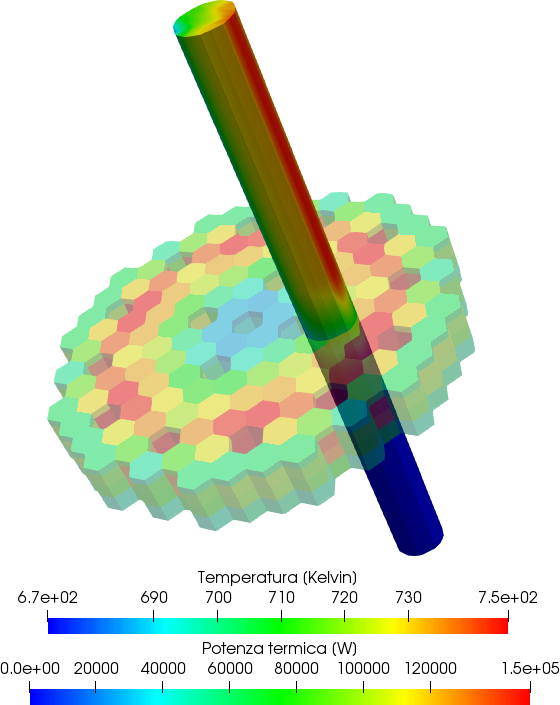
\includegraphics[scale=0.2]{../../thesis/figure/result_tred/morenew/tempassurda}
%   \end{figure}
%    
%   \end{center}
% 
%   \end{column}
%   \begin{column}{0.48\textwidth}
%   \begin{figure}
%    \centering
% %       \includegraphics[scale=0.30]{../../thesis/figure/result_tred/pacman}
%    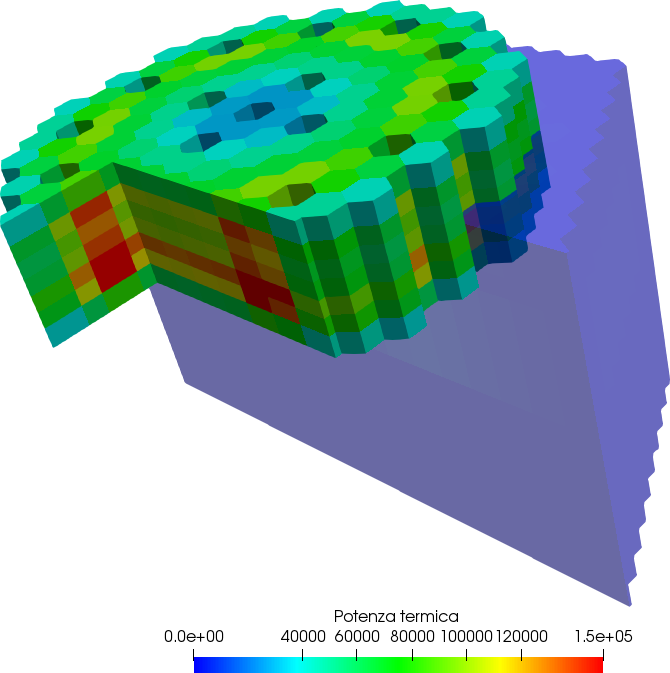
\includegraphics[scale=0.2]{../../thesis/figure/result_tred/new/tred7-pw.png}
%   \end{figure}
%    % % % %      \begin{center}
% % % % %        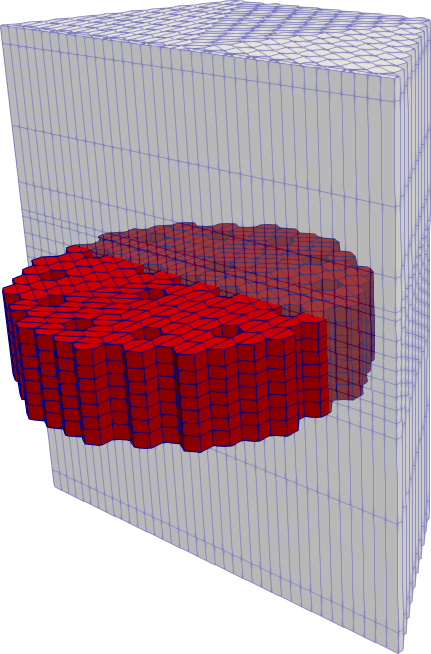
\includegraphics[scale=0.3]{../../thesis/figure/result_tred/new/tred-reactor}
% % % % %    \end{center}
%   \end{column}
% 
%  \end{columns}
% 
% \end{frame}





 %%%%%%%%%%%%%%%%%%%%%%%%%%%%%%%%%%%%%%%%%%%%%%%%%%%%%%%%%
\subsection{Reattore Nucleare}
 \begin{frame}
 \vspace{0.4cm}
 \frametitle{ALFRED (Advanced Lead Fast REactor Demonstrator)}
%  \framesubtitle{Advanced Lead Fast REactor Demonstrator}
\begin{center}
\large
 Progetto europeo di reattore nucleare (300 MW$_{th}$) che ha il ruolo di dimostrare la 
 \textbf{fattibilità della tecnologia dei reattori veloci raffreddati a piombo}, 
 i quali hanno caratteristiche di \underline{affidabilità} e di \underline{sostenibilità}.
\end{center}
 \begin{center}
 \begin{figure}
 \centering
 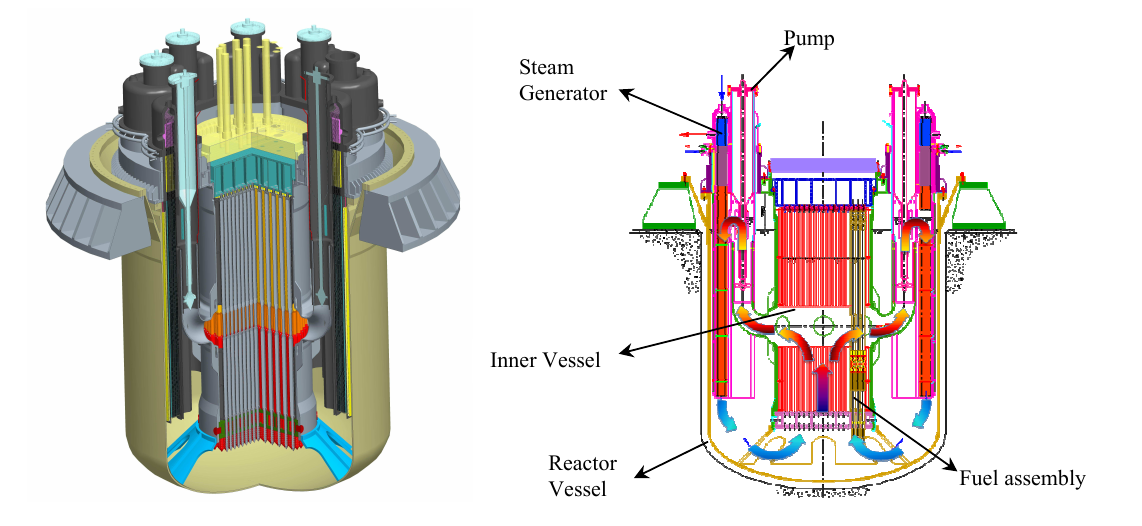
\includegraphics[scale=0.33]{../../thesis/figure/reactor/alfred.png}
 \end{figure}
 \end{center}
 
 \begin{center}
 \begin{itemize}
  \item Combustibile ossidi misti di uranio e di plutonio (MOX)
  \item Refrigerante Piombo Liquido
 \end{itemize}
 \end{center}
 
 \end{frame}
 
 %%%%%%%%%%%%%%%%%%%%%%%%%%%%%%%%%%%%%%%%%%%%%%%%%%%%%%%%%
 \begin{frame}
  \frametitle{Caratteristiche dei Reattori Veloci}
  \vspace{0.4cm}
  \begin{center}
  \begin{itemize}
  \item Prevalenza di reazioni di \textbf{fissione veloce}
  \item Ogni evento di fissione veloce libera \textbf{più neutroni} rispetto alle fissioni termiche
%   \item Tuttavia le reazioni di fissione alle alte energie sono \textbf{meno probabili} rispetto alle basse energie 
  \item \textbf{Maggiori assorbimenti} da parte degli isotopi fertili che trasmutano in isotopi fissili
  \begin{equation*}
 ^{238}_{92}U + ^{1}_{0}n \, \longrightarrow ^{239}_{92}U  \xrightarrow{\beta^-}
 \, ^{239}_{93}Np  \xrightarrow{\beta^-} \, ^{239}_{94}Pu
 \end{equation*}
  \item \textbf{Maggiore compattezza} dovuta all'assenza del moderatore di neutroni
 \end{itemize}
 \begin{block}{Sostenibilità}
 Capacità di \textbf{\textcolor{red}{autofertilizzazione}} del combustibile (Breeder Reactor), con la possibilità di generare più combustibile di quello che brucia
 \end{block}
 
 \end{center}
 \end{frame}

 
 %%%%%%%%%%%%%%%%%
% % %  \begin{frame}
% % %  
% % %  \frametitle{Reattori veloci raffreddati al piombo}
% % %   \begin{minipage}[c]{0.48\linewidth} 
% % %  \begin{center}
% % %  \begin{figure}
% % %  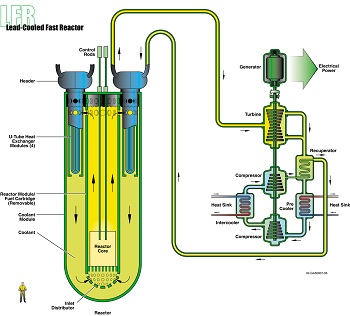
\includegraphics[scale=2.2]{../../thesis/figure/reactor/lfr.jpg}
% % %  \end{figure}
% % %  \end{center}
% % %  \end{minipage}\hfill
% % %  
% % %  \end{frame}
 %%%%%%%%%%%%%%%%%%%%%%%%%%%%%%%%%%%
 \begin{frame}
 \frametitle{Vantaggi e svantaggi del piombo liquido come refrigerante}
 \vspace{0.5cm}
 % \begin{minipage}[c]{0.48\textwidth} 
 \begin{block}{Vantaggi}
 \begin{itemize}
 \item[\checkmark] Mantiene uno spettro veloce dei neutroni
 \item[\checkmark] Ottime proprietà termodinamiche
 \item[\checkmark] Alta temperatura di ebollizione ($T_{ebollizione}=1739 ^\circ C$)
 \item[\checkmark] Bassa reattività con acqua o aria (inerte)
 \item[\checkmark] Schermaggio delle radiazioni dovute a decadimenti
 \end{itemize}
 \end{block}
 
 %  \end{minipage}\hfill
 
% \begin{minipage}[c]{0.48\textwidth} 
 \begin{block}{Svantaggi}
 \begin{itemize}
 \item[\textbf{$\times$}] Elevata tendenza ad essere corrosivo nei confronti dell'acciaio
 \item[\textbf{$\times$}] Opacità del piombo causa problematiche per l'ispezione e il monitoraggio
 \item[\textbf{$\times$}] Sistema ausiliario per mantenere il piombo liquido ($T_{fusione}=327.5 ^\circ C$)
 \end{itemize}
 \end{block}
 % \end{minipage}\hfill
 \end{frame}
 
 \begin{frame}
 \frametitle{Scopo della tesi}
 
%  \vspace{0.8cm}

  \begin{columns}
  \begin{column}{0.5\textwidth}
  
 \begin{block}{}
 \begin{itemize}
 \item Generare le \textbf{sezioni d'urto macroscopiche} mediate sulla composizione e sull'energia, partendo dalle librerie dei dati nucleari
 \item Modellare il reattore nucleare ALFRED
 \item Implementare il modello all'interno della piattaforma numerica
 \item Consentire l'accoppiamento tra i codici di neutronica e i codici di termoidraulica
 \item Simulare il comportamento multifisico
 \end{itemize}
 \end{block}
 
  \end{column}
  \begin{column}{0.44\textwidth}
  \vspace{0.8cm}
  \begin{figure}
   \centering
%       \includegraphics[scale=0.30]{../../thesis/figure/result_tred/pacman}
   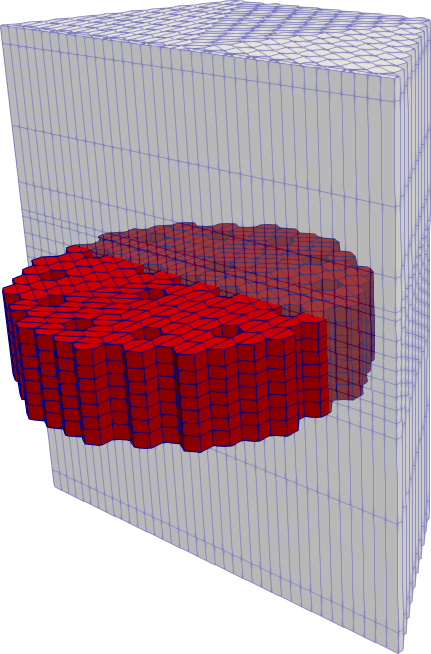
\includegraphics[scale=0.28]{../../thesis/figure/result_tred/new/tred-reactor}
  \end{figure}
   % % % %      \begin{center}
% % % %        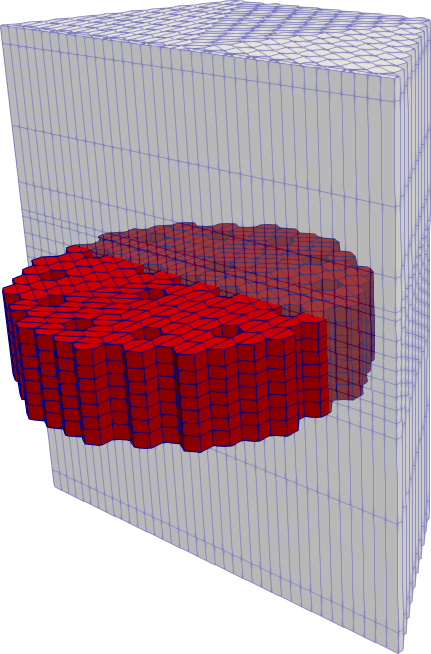
\includegraphics[scale=0.3]{../../thesis/figure/result_tred/new/tred-reactor}
% % % %    \end{center}
  \end{column}

 \end{columns}
% 
 
\end{frame} 
 %%%%%%%%%%%%%%%%%%%%%%%%%%%%%%%%%%%%%%%%%%%%%%%%%%%%%%%%%


\section{Piattaforma Numerica}

% 
\begin{frame}
\frametitle{Piattaforma Numerica}

\begin{center}
 \vspace{0.3cm}
 %     \begin{center}
%      
%    \large La piattaforma numerica  semplificato e versatile}
%    che permette l'integrazione e l'accoppiamento dei codici computazionali di \textbf{\textcolor{bleudefrance}{neutronica}} e
%    di \textbf{\textcolor{mygreen}{termoidraulica}}.
%    
%     \end{center}
 La piattaforma numerica consiste in un \textbf{ambiente computazionale}, basato sul progetto \textit{Salom\'e}, e permette la  
%  coordinare i codici computazionali
 \textbf{gestione} e \textbf{condivisione} delle strutture dati 
 tra i moduli di \textbf{\textcolor{bleudefrance}{neutronica}} e di \textbf{\textcolor{mygreen}{termoidraulica}} \\
 \end{center}
%  \vspace{0.5cm}
%  \begin{center}
  \begin{columns}\hspace{0.5cm}
 \begin{column}{0.42\textwidth}
 \begin{block}{Obiettivo}
%  \begin{center}
   \begin{itemize}
    \item Consentire l'\textbf{accoppiamento} tra la 
     neutronica
     e la termoidraulica
    \item Ottenere la soluzione di un \textbf{problema multifisico} in un ambiente semplificato e versatile
   \end{itemize}
  \end{block}
%   \begin{block}{Scopo dell'accoppiamento neutronico-termoidraulico}
%   \begin{itemize}
%   \item Scambiare la potenza termica ottenuta dal modulo di neutronica con il
%   modulo di termoidraulica
%   \item A sua volta, il modulo di termoidraulica restituisce la distribuzione del campo di temperatura
%   al modulo di neutronico al fine di correggere il flusso neutronico a seguito delle variazioni di tempertura
%   \end{itemize}
%   \end{block}
\end{column}
\begin{column}{0.5\textwidth}
\begin{minipage}{\textwidth}
\begin{tikzpicture}[overlay]
 \node[xshift=25mm,yshift=32mm, text width = 4cm](sigma) {\textbf{\textcolor{mygreen}{$T_f,T_c$}}};
 \node[xshift=45mm,yshift=-2mm, text width = 4cm](sigma) {\textbf{\textcolor{bleudefrance}{$\phi$, $P_{th}$}}};
 \node[xshift=63mm,yshift=30mm, text width = 4cm](TF) {\textbf{\textcolor{red}{$\Sigma_f,\Sigma_a,\Sigma_s$}}};
\end{tikzpicture}
\scalebox{.7}{\smartdiagramset{set color list={red, bleudefrance, mygreen}, }\smartdiagram[circular diagram:clockwise]{Database Nucleare (Dragon), Simulazione Neutronica (Donjon), Analisi Termo Idraulica (FEMuS)}}
\end{minipage}
\end{column}
\end{columns}
\vspace{0.2cm}
\begin{center}
 Entrambi i codici ottengono la soluzione numerica attraverso \\ il \textbf{metodo degli elementi finiti}
\end{center}


\end{frame}
% %%%%%%%%%%%%%%%%%%%%%%%%%%%%%%%%%%%%%%%%%%%%%%%%%%%%%%%%%%
% \begin{frame}
% Equazione della diffusione neutronica
% \begin{multline*}
%  -\nabla \cdot(D_g(\vec{r})\nabla \phi_g(\vec{r}))+\Sigma_g(\vec{r})\phi_g(\vec{r})=\\
%  =\sum_{h=1}^G \Sigma_{h \rightarrow g}(\vec{r}) 
% \phi_h(\vec{r})+\frac{\chi_g(\vec{r})}{k_{eff}} \sum_{h=1}^G \nu 
% \Sigma_{f,h}(\vec{r})\phi_h(\vec{r})   \,.
% \end{multline*}
% Equazione del calore
% \begin{equation*}
%  \rho c_v\frac{dT}{dt}=\nabla \cdot (\kappa \nabla T) + \mu \Phi + \rho 
% \vec{g}\cdot \vec{\upsilon} + \dot{Q} \,.
% \end{equation*}
% \end{frame}
% %%%%%%%%%%%%%%%%%%%%%%%%%%%%%%%%%%%%%%%%%%%%%%%%%%%%%%%%%%5
\subsection{Codice di Neutronica}

\begin{frame}
 \frametitle{Modulo di Neutronica}
 
 \begin{center} \vspace{0.2cm} 
 \begin{block}{}
   \begin{itemize}
     \item \textbf{\textcolor{red}{Dragon}}: Codice di cella risolve le \textbf{equazioni del trasporto multigruppo} 
     allo scopo
     di ottenere le \textit{sezioni d'urto macroscopiche $\Sigma_i$}  e di generare il \textbf{database nucleare}
   \end{itemize}
   \end{block}
   \begin{block}{}
   \begin{itemize}
    \item \textbf{\textcolor{bleudefrance}{Donjon}}: Codice di reattore che simula il comportamento dei neutroni sull'intero
          reattore, ottenendo la distribuzione di \textbf{flusso neutronico} $\phi_g$ e di \textbf{potenza termica}. 
%           attraverso la risoluzione
% 	  dell'equazione di diffusione o di equazioni $SP_N$.
      \end{itemize}	  
  \end{block}

   \underline{Equazione multigruppo della diffusione neutronica}
\begin{multline*}
 -\nabla \cdot(D_g(\vec{r})\nabla \phi_g(\vec{r}))+\Sigma_g(\vec{r})\phi_g(\vec{r})=\\
 =\sum_{h=1}^G \Sigma_{h \rightarrow g}(\vec{r}) 
\phi_h(\vec{r})+\frac{\chi_g(\vec{r})}{k_{eff}} \sum_{h=1}^G \nu 
\Sigma_{f,h}(\vec{r})\phi_h(\vec{r})   \,.
\end{multline*}
  \end{center}

  \end{frame}
 
 \subsection{Codice di Termoidraulica}
 
 \begin{frame}
  \frametitle{Modulo di Termoidraulica}
   \begin{center}
%    \vspace{0.5cm}
   \begin{block}{}
   \begin{itemize}
    \item \textbf{\textcolor{mygreen}{FEMuS}}: Codice CFD che risolve le equazioni di termofluidodinamica
    con possibilità di aggiungere modelli di turbolenza.   
    \end{itemize}
      \end{block}
      
    \underline{Equazione del calore per fluidi incomprimibili}
    \begin{equation*}
 \rho c \frac{dT}{dt}=\nabla \cdot (\kappa \nabla T) + \mu \Phi + \rho 
\vec{g}\cdot \vec{\upsilon} + \dot{Q}_{neutronica} 
\end{equation*}



 \underline{Proprietà termodinamiche del piombo}
 \begin{table}[!htb]
\centering
 \begin{tabular}{lccc}
\hline
Parametro & Simbolo & Unità & Valore \\
\hline
Densità & $\rho$ & kg/m$^3$ & 11340 \\
Conducibilità termica & $\kappa$ & W/(m$\cdot$K) & 35 \\
Calore specifico & $c$ & J/(kg$\cdot$K) & 129 \\
Viscosità dinamica & $\mu$ & Pa$\cdot$s & 0.001844 \\
\hline
\end{tabular}
\end{table}

  \begin{itemize}
 \item Non è necessario risolvere Navier-Stokes (Canali chiusi)
 \item Conducibilità termica mediata su tutti i materiali dell'assembly 
\end{itemize}
%   \item \begin{block}{FEMuS}
%          Codice di termoidraulica che risolve le principali equazioni di termodinamica.
%         \end{block}
%   \end{itemize}
%   In supporto alla neutronica, il

 \end{center}

\end{frame}

%%%%%%%%%%%%%%%%%%%%%%%%%%%%%%%%%%%%%%%%%%%%%%%%%%%%%%%%%%%%%%%%%%%%

\begin{frame}
\frametitle{Logica dell'accoppiamento neutronico-termoidraulico}
\vspace{0.1cm}
\begin{columns}\hspace{0.5cm}
 \begin{column}{0.35\textwidth}
 
% 
\begin{center} 
  \begin{itemize}
   \item Librerie dati nucleari \textbf{\textcolor{orange}{JEFF-3.1.2-SHEM315}}
   \item Codice di cella\\ \textbf{\textcolor{red}{Dragon}}
   \item Codice di reattore\\ \textbf{\textcolor{bleudefrance}{Donjon}}
   \item Codice di termoidraulica \textbf{\textcolor{mygreen}{FEMuS}}
  \end{itemize}
  
\end{center}
%  \end{block}
 \end{column}

 \begin{column}{0.72\textwidth}
  \begin{center}
 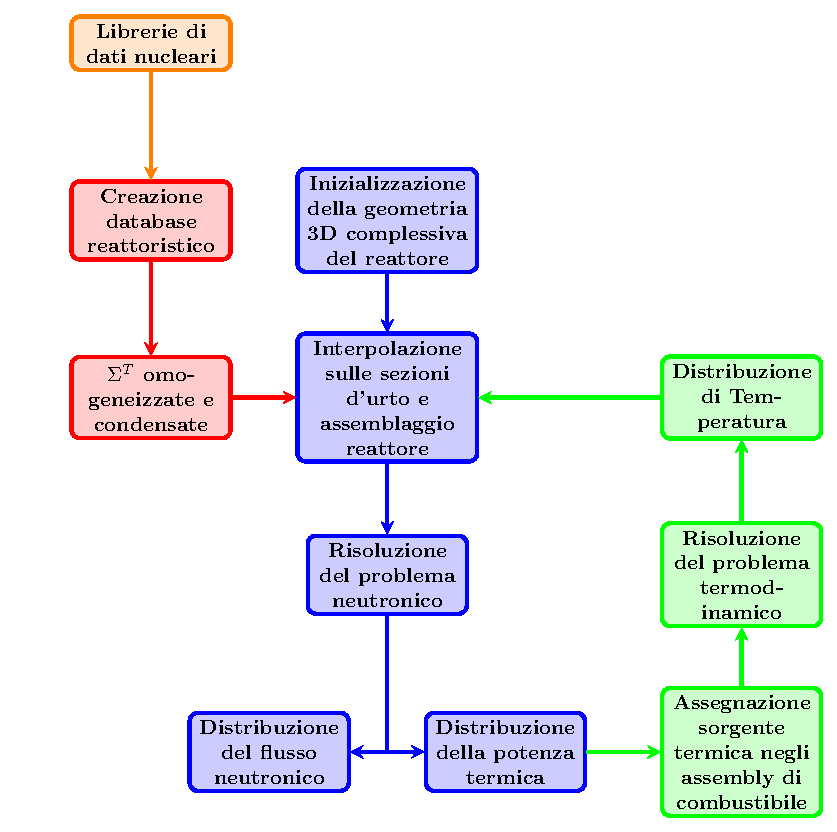
\includegraphics[scale=0.55]{../../thesis/figure/flowchart/dataflow_platform}
 \end{center}
 \end{column}
 \end{columns}

\end{frame}

% % % % %  %%%%%%%%%%%%%%%%%%%%%%%%%%%%%%%%%%%%%%%%%%%%%%%%%%%%%%%%%%%%%%%%%%%%%%
% % % % %  \section{Modellazione del reattore}
% % % % %  \begin{frame}
% % % % %  \frametitle{Creazione del database nucleare}
% % % % %  \vspace{0.5cm}
% % % % %  
% % % % %  \begin{center}
% % % % %   Il \textbf{database nucleare} contiene le informazioni sulle sezioni d'urto macroscopiche $\Sigma_T$,
% % % % %   omogeneizzate su ciascuna cella e condensate a 33 gruppi di energia, degli elementi che compongono il
% % % % %   reattore.
% % % % %  \end{center}
% % % % %   \begin{columns}
% % % % %   
% % % % %     \begin{column}{0.6\textwidth}
% % % % % %       \begin{center}
% % % % % %     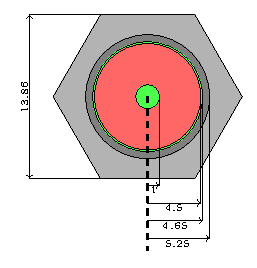
\includegraphics[scale=1]{../../thesis/figure/itex/unitcells_wq}
% % % % % %     
% % % % % %    \end{center}
% % % % %      Parametri per le interpolazione
% % % % %      \begin{itemize}
% % % % %       \item Temperatura del combustibile $T_f$
% % % % %       \item Temperatura del refrigerante $T_c$
% % % % %       \item Tempo relativo al bruciamento $t_{burnup}$
% % % % %      \end{itemize}
% % % % % 
% % % % % 
% % % % %    
% % % % %   \end{column}
% % % % %   
% % % % % 
% % % % %   
% % % % %   \begin{column}{0.4\textwidth}
% % % % %    \begin{center}
% % % % %     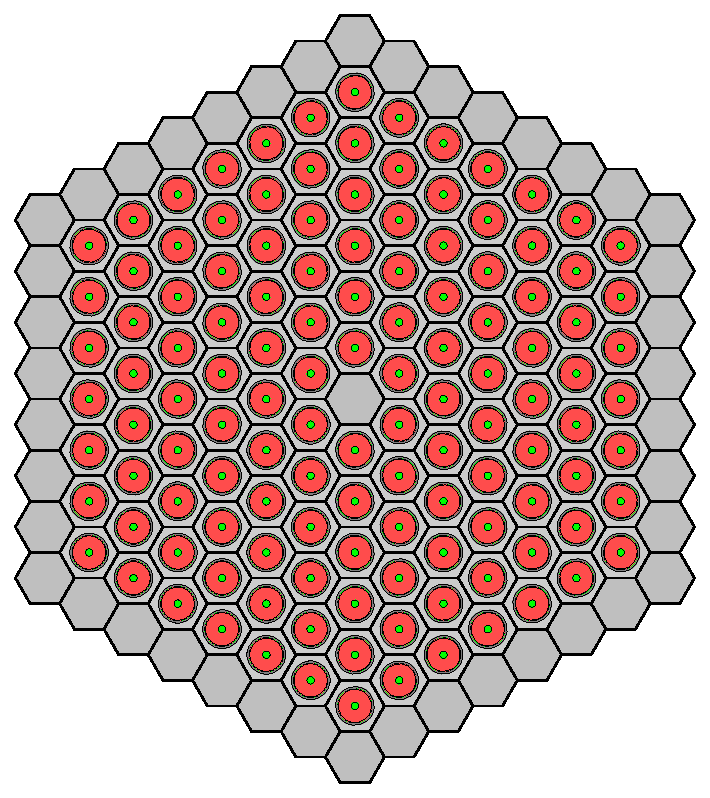
\includegraphics[scale=0.26]{../../thesis/figure/itex/fassembly}\\
% % % % %     Assembly di combustibile
% % % % %    \end{center}
% % % % %    \end{column}
% % % % %    
% % % % %   
% % % % %   
% % % % %  \end{columns}
% % % % %  \begin{block}{}
% % % % %    \begin{center}
% % % % %   La sua realizzazione permetterà al codice di reattore \textcolor{bleudefrance}{\textbf{Donjon}} di correggere le sezioni d'urto a seguito delle variazioni
% % % % %   di temperatura.
% % % % %  \end{center}
% % % % % 
% % % % %  \end{block}
% % % % %  \end{frame}
% % % % %  
%%%%%%%%%%%%%%%%%%%%%%%%%%%%%%%%%%%%%%%%%%%%%%%%%%%%%%%%%%%%%%%%%%%%%%%%%%%%%%%%%%%%%%%%%%%%%%%%%%%%%%%%%%%%% 
% % % %  %%%%%%%%%%%%%%%%%%%%%%%%%%%%%%%%%%%%%%%%%%%%%%%%%%%%%%%%%%%
% % % %  \begin{frame}
% % % %  
% % % %     \begin{columns}
% % % %   
% % % %     \begin{column}{0.6\textwidth}
% % % %  \small{
% % % %  \begin{tabular}{lcc}
% % % % \hline
% % % % Parametro & Unità & Valore \\
% % % % \hline
% % % % N$^\circ$ totale di esagoni & - & 169 \\
% % % % N$^\circ$ barre di combustibile & - & 126 \\
% % % % N$^\circ$ elementi di acciaio & - & 43 \\
% % % % Lato di un esagono & mm & 8.00208 \\
% % % % Apotema di un esagono & mm & 6.93 \\
% % % % Distanza tra barre di combustibile & mm & 13.86 \\
% % % % Raggio barra di combustibile & mm & 5.25 \\
% % % % \hline
% % % % \end{tabular}
% % % %    }
% % % %   \end{column}
% % % %   
% % % % 
% % % %   
% % % %   \begin{column}{0.4\textwidth}
% % % %   
% % % %    \begin{center}
% % % %     \underline{Esagono di combustibile}
% % % %     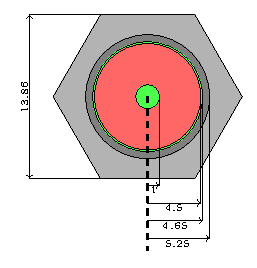
\includegraphics[scale=1.2]{../../thesis/figure/itex/unitcells_wq}\\
% % % % 
% % % %    \end{center}
% % % %    \end{column}
% % % %    
% % % %   
% % % %   
% % % %  \end{columns}
% % % %   
% % % %   
% % % %  \end{frame}
% % % % 
% % % %  %%%%%%%%%%%%%%%%%%%%%%%%%%%%%%%%%%%%%%%%%%%%%%%%%%%%%%%%%%%
 \begin{frame}
 \frametitle{Geometria complessiva del reattore}
 \vspace{0.3cm}
 \begin{columns}
  
  \begin{column}{0.48\textwidth}
%   \begin{itemize}
%    \item[-] \textcolor{yellow}{$\circ$} Combustibile MOX arricchito al \underline{20.5$\%$}
%    \item[-] \textcolor{red}{$\circ$} Combustibile MOX arricchito al \underline{26.2$\%$}
%    \item[-] \textcolor{green}{$\circ$} Barre di controllo
%    \item[-] \textcolor{purple}{$\circ$} Barre di sicurezza
%   \end{itemize}
   \begin{center}
   
  \underline{Sezione radiale del nocciolo}
    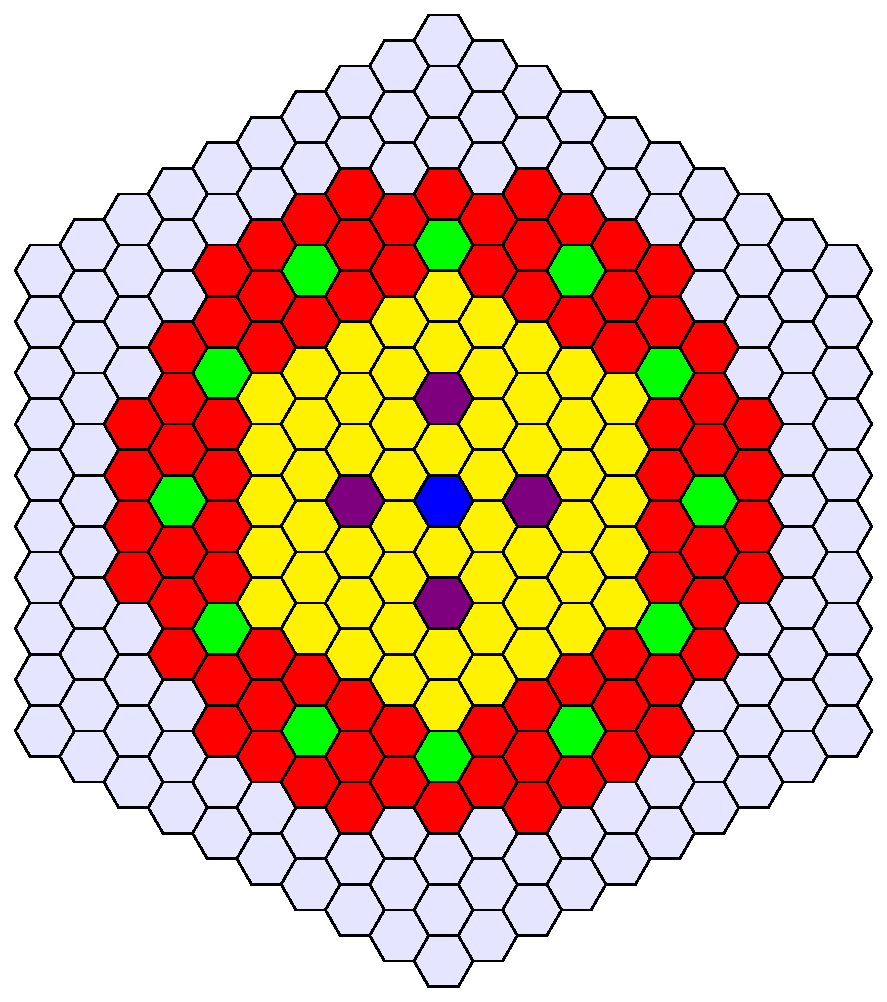
\includegraphics[scale=0.3]{../../thesis/figure/itex/hexagon}
   \end{center}

  \end{column}
  
    \begin{column}{0.48\textwidth}
     \begin{center}
     \underline{Sezione assiale del reattore}
    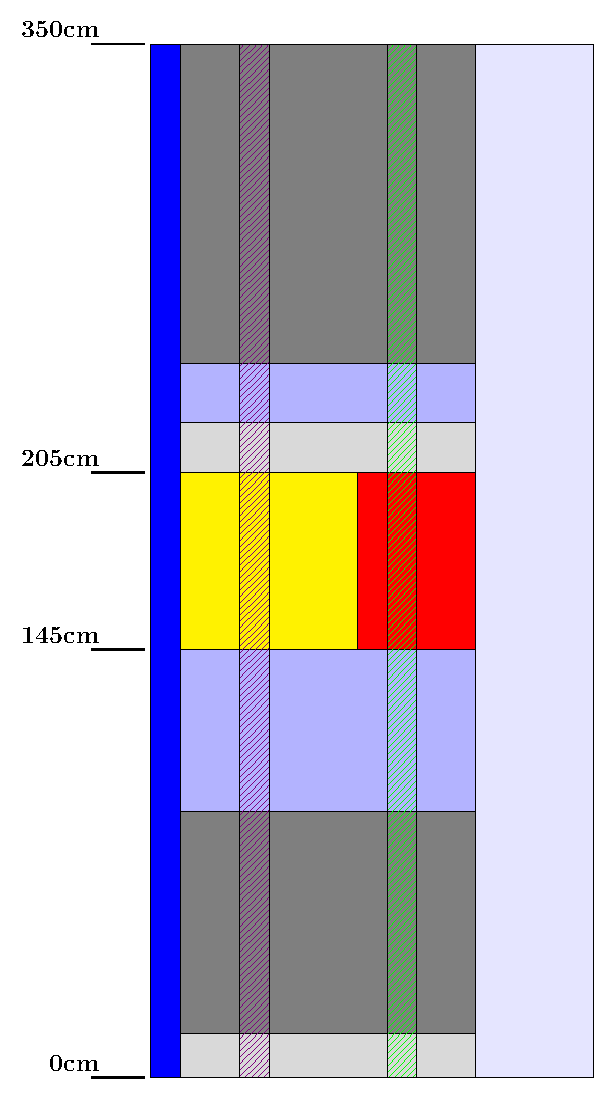
\includegraphics[scale=0.28]{../../thesis/figure/itex/rectangle_wq}
   \end{center}
   

  \end{column}
  
 \end{columns}
 \vspace{0.3cm}
 \begin{center}
 \begin{itemize}
  \item  Arricchimento combustibile MOX interno {\underline{20.5$\%$}} (in giallo), 
    esterno {\underline{26.2$\%$} (in rosso)}
  \item 12 barre di controllo (in verde) e 4 di sicurezza (in viola)
 \end{itemize}
 \end{center}

 \end{frame}
 %%%%%%%%%%%%%%%%%%%%%%%%%%%%%%%%%%%%%%%%%%%%%%%%%%%%%%%%%%%%%
 
  %%%%%%%%%%%%%%%%%%%%%%%%%%%%%%%%%%%%%%%%%%%%%%%%%%%%%%%%%%%%%
% % % %  \begin{frame}
% % % %  \frametitle{Modellazione complessiva del reattore}
% % % %  \begin{columns}
% % % %   
% % % %   \begin{column}{0.48\linewidth}
% % % %      \begin{center}
% % % %   \underline{Sezione assiale del reattore}
% % % %     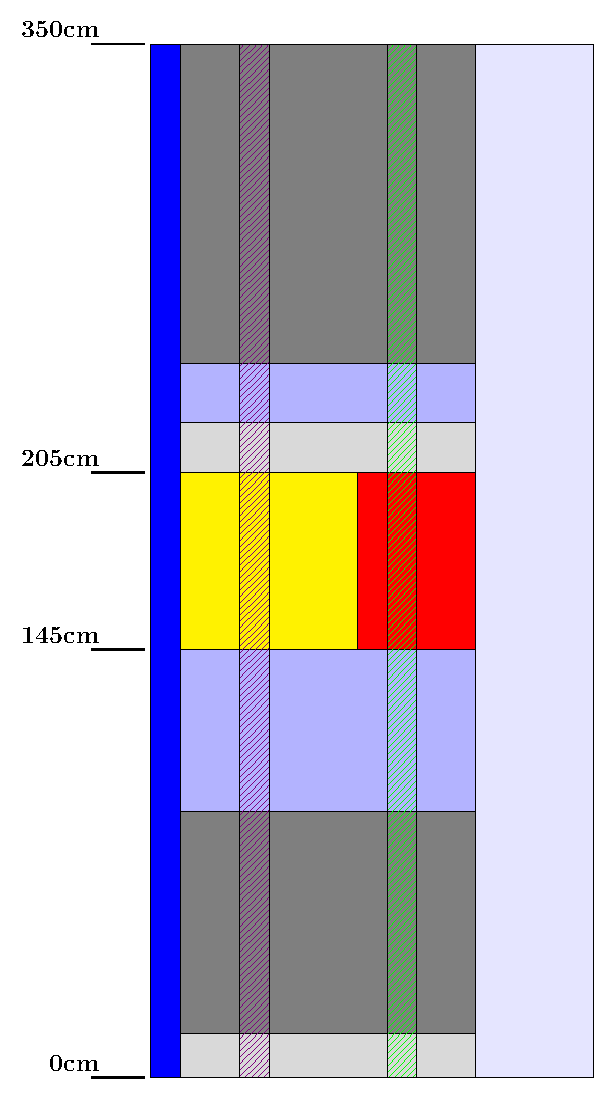
\includegraphics[scale=0.35]{../../thesis/figure/itex/rectangle_wq}
% % % %    \end{center}
% % % %   \end{column}
% % % %   
% % % %     \begin{column}{0.48\linewidth}
% % % %      \begin{center}
% % % %      \underline{Reattore tridimensionale}
% % % %        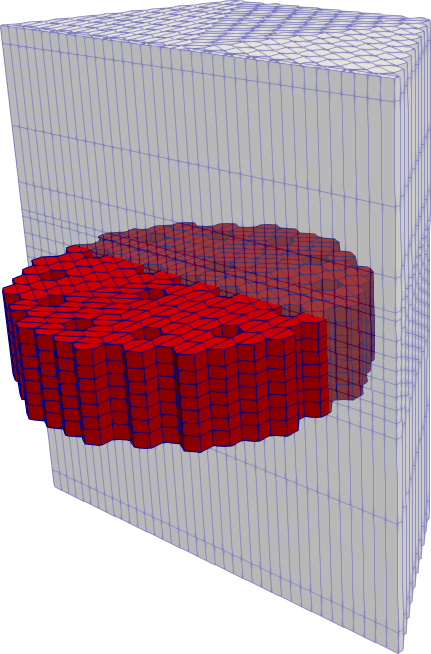
\includegraphics[scale=0.3]{../../thesis/figure/result_tred/new/tred-reactor}
% % % %    \end{center}
% % % %   \end{column}
% % % %   
% % % %  \end{columns}
% % % %  



% % % % %  \end{frame}
 %%%%%%%%%%%%%%%%%%%%%%%%%%%%%%%%%%%%%%%%%%%%%%%%%%%%%%%%%%%%%
%  \begin{frame}
%  \frametitle{Codice di termoidraulica}
%  \begin{columns}
%   
%   \begin{column}{0.48\textwidth}
%      \begin{center}
%     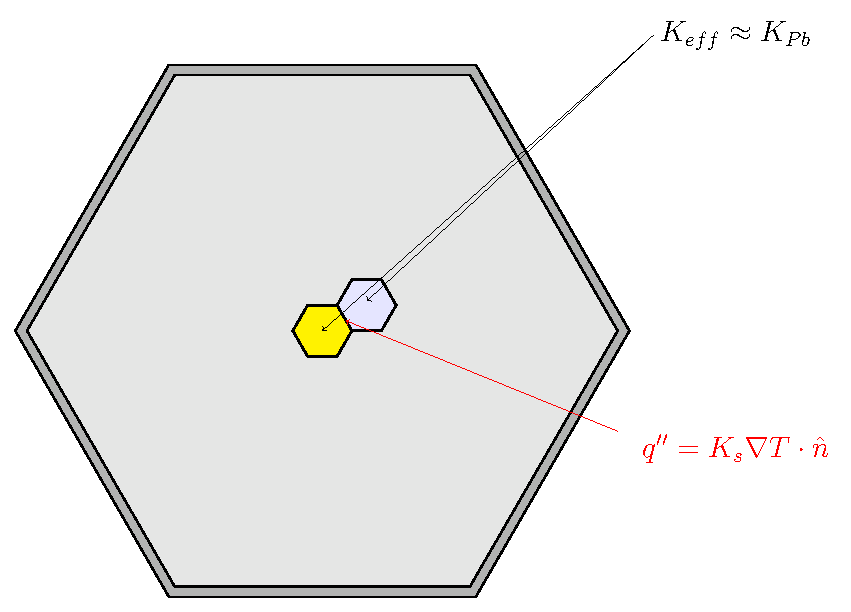
\includegraphics[scale=0.4]{../../thesis/figure/itex/tempeq}
%    \end{center}
%   \end{column}
%   
%     \begin{column}{0.48\textwidth}
%      \begin{center}
%     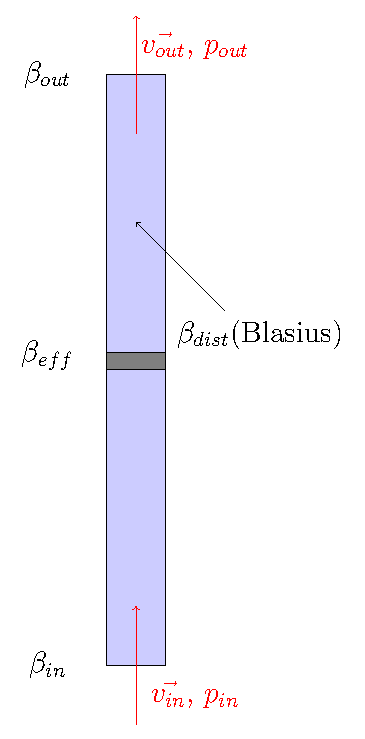
\includegraphics[scale=0.35]{../../thesis/figure/itex/canale}
%    \end{center}
%   \end{column}
%   
%  \end{columns}
%  \end{frame}

\section{Risultati}
%  \begin{frame}
% \frametitle{Distribuzione di flusso neutronico}
% \begin{figure}[!htb]
% \centering
% \subfigure[Sezione con barre inserite]
% {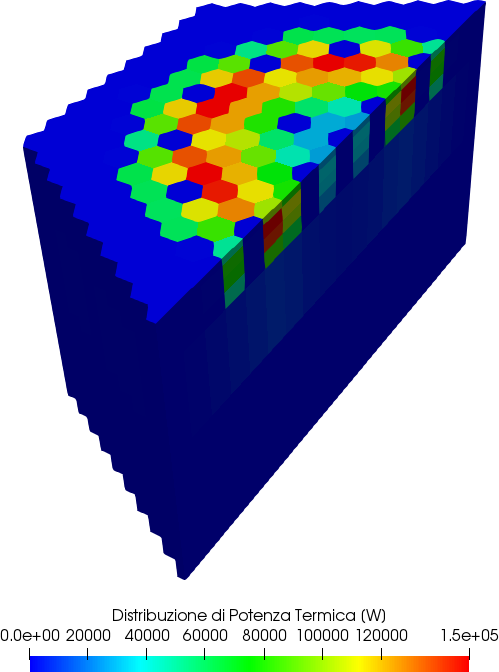
\includegraphics[height=0.28\textheight]{../../thesis/figure/result_tred/morenew/pw-clip-insert1.png}}
% \hspace{1.2cm}
% \subfigure[Nocciolo con barre inserite]
% {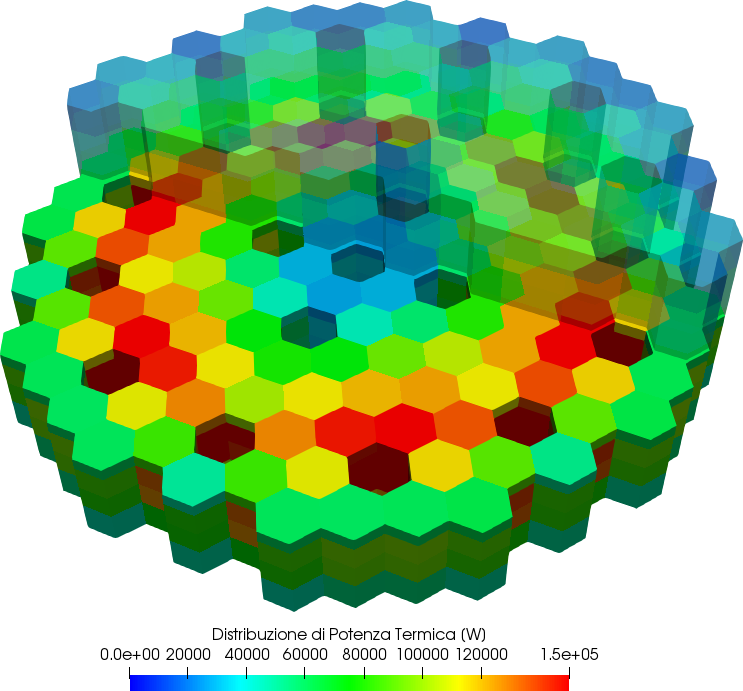
\includegraphics[height=0.28\textheight]{../../thesis/figure/result_tred/morenew/pw-trashold-insert1.png}}\\
% \subfigure[Sezione con barre estratte]
% {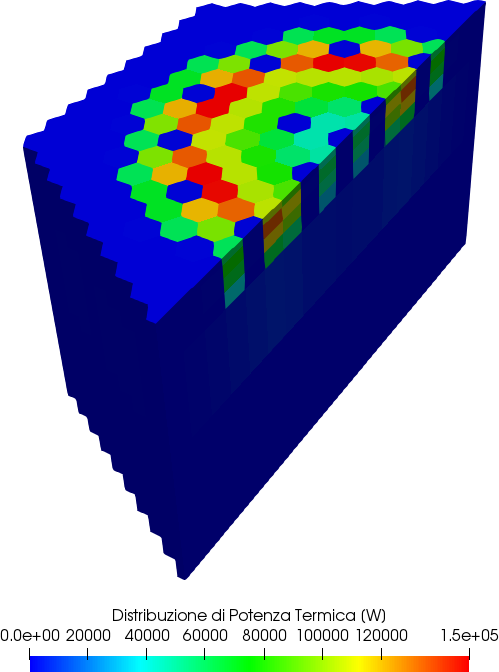
\includegraphics[height=0.28\textheight]{../../thesis/figure/result_tred/morenew/pw-clip-exstract1.png}}
% \hspace{1.2cm}
% \subfigure[Nocciolo con barre estratte]
% {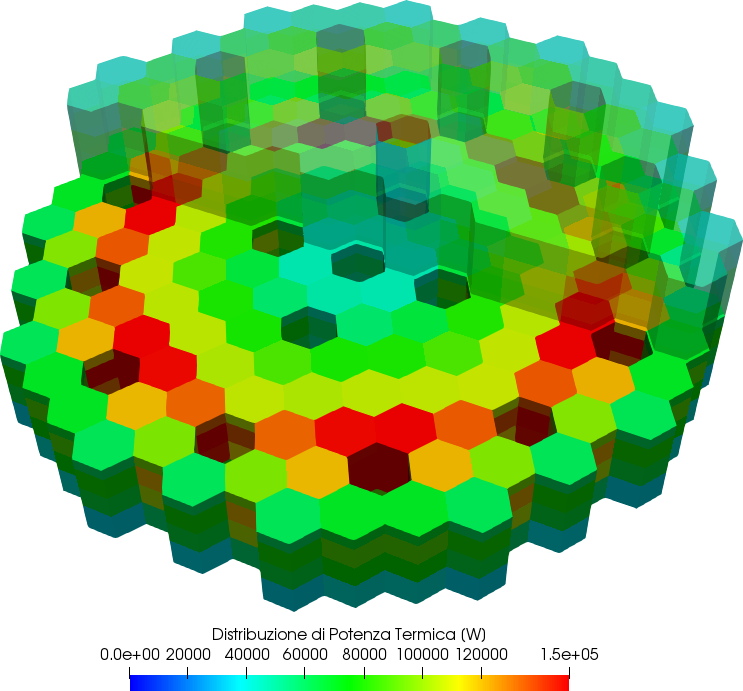
\includegraphics[height=0.28\textheight]{../../thesis/figure/result_tred/morenew/pw-trashold-exstract1.png}}
% \end{figure}
% \end{frame}
%  \begin{frame}
% \frametitle{Distribuzione di flusso neutronico}
% \begin{figure}[!htb]
% \centering
% \subfigure[Sezione con barre inserite]
% {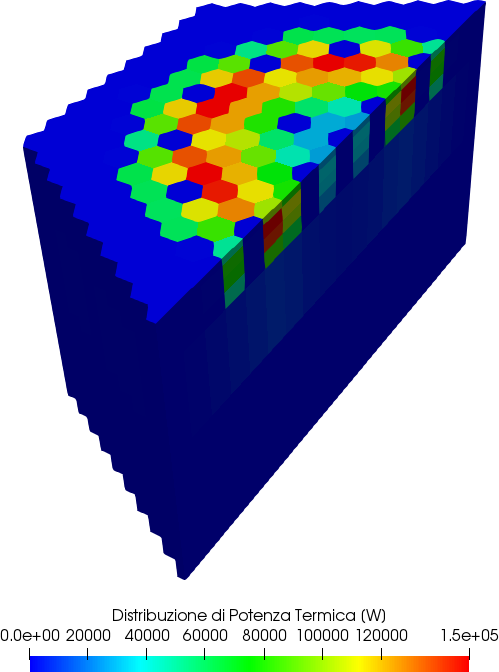
\includegraphics[height=0.28\textheight]{../../thesis/figure/result_tred/morenew/pw-clip-insert1.png}}
% \hspace{1.2cm}
% \subfigure[Nocciolo con barre inserite]
% {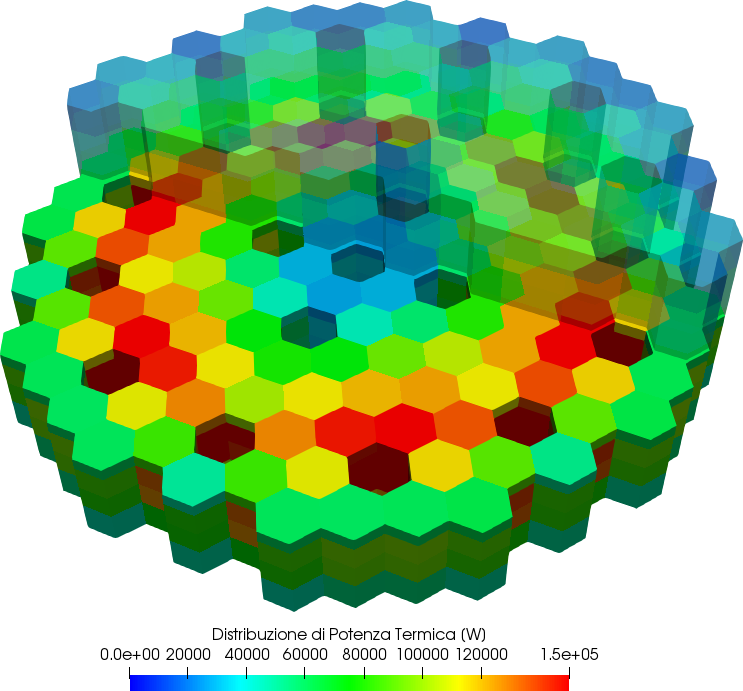
\includegraphics[height=0.28\textheight]{../../thesis/figure/result_tred/morenew/pw-trashold-insert1.png}}\\
% \subfigure[Sezione con barre estratte]
% {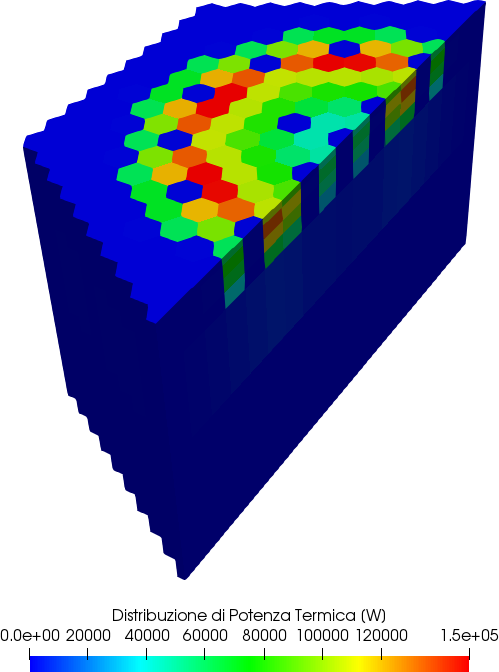
\includegraphics[height=0.28\textheight]{../../thesis/figure/result_tred/morenew/pw-clip-exstract1.png}}
% \hspace{1.2cm}
% \subfigure[Nocciolo con barre estratte]
% {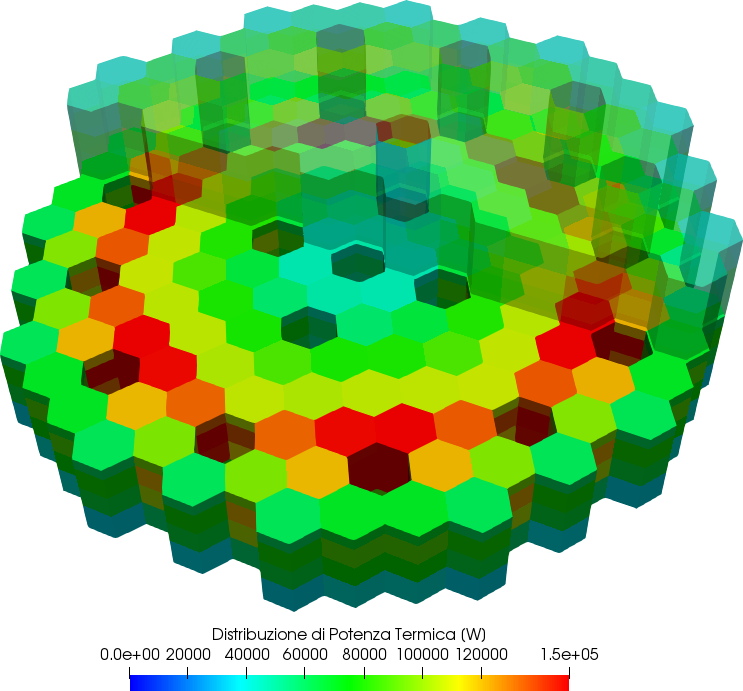
\includegraphics[height=0.28\textheight]{../../thesis/figure/result_tred/morenew/pw-trashold-exstract1.png}}
% \end{figure}
% \end{frame}
% 
\begin{frame}
\frametitle{Validazione Neutronica}
\vspace{0.4cm}
\begin{center}

  Confronto tra i valori della costante moltiplicativa effettiva $k_{eff}$ 
  tra il codice deterministico \textbf{\textcolor{blue}{Donjon}} e il codice probabilistico
  \textbf{MCNPX} effettuato in un altro studio
  
  
 \begin{center}
 \begin{tabular}{l|cc|cc}
\hline
Tempo [Giorni] & $k_{eff}$ Donjon [-] & & $k_{eff}$ MCNPX [-] & \\
$t_{burnup}$ & Barre Estratte & Inserite & Barre Estratte & Inserite \\
\hline
0   & 1.1177  & 1.0794  & 1.0804 & 1.0525  \\
365 & 1.0887  & 1.0520  & 1.0510 & 1.0229   \\
730 & 1.0624  & 1.0272  & 1.0247 & 0.9964   \\
1095 & 1.0384  & 1.0001 & 0.9988  & 0.9703 \\
\hline
\end{tabular}
  \end{center}
  \begin{figure}
   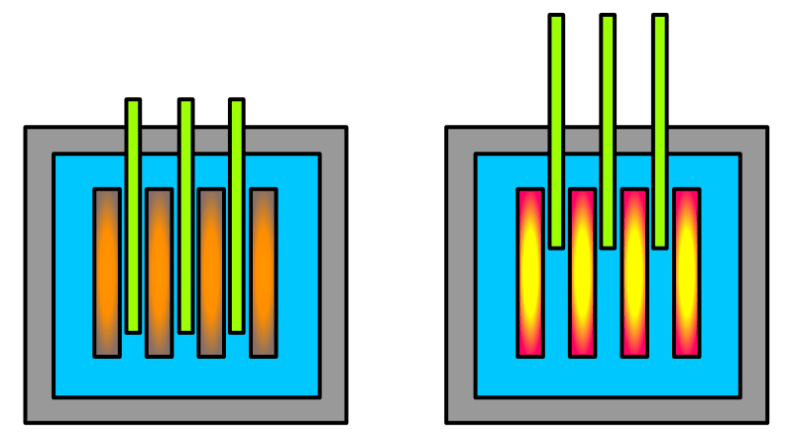
\includegraphics[scale=0.15]{../barre-di-controllo}
  \end{figure}
 inserite\quad \quad  \quad estratte
\end{center}  
\end{frame}
% %    %%%%%%%%%%%%%%%%%%%%%%%%%%%%%%%%%%%%%%%%%%%%%%%%%%%%%%%%%%%%%%
% % \begin{frame}
% % \frametitle{Validazione Neutronica}
% % Confronto tra i valori della costante moltiplicativa effettiva $k_{eff}$ 
% %   tra il caso deterministico di \textcolor{blue}{Donjon} e il caso probabilistico
% %   di MCNPX, effettuato in un altro studio.
% %  \begin{columns}
% %   \begin{column}{0.5\textwidth}
% %    %%%%%%%%%%%%%%%%%%%%%%%%%%%%%%%%%%%%%%%%%%%%%%%%%%%%%%%%%%%%%%
% % %   \begin{equation*}
% % %    k_{eff}=\frac{popolazione neutronica del}{×}
% % %   \end{equation*}
% % 
% % 
% %   \end{column}
% % 
% %   \begin{column}{0.4\textwidth}
% %   \begin{center}
% %       \begin{table}
% %  \begin{tabular}{lcc}
% % \hline
% % Tempo  & Donjon  &  MCNPX \\
% % $[$giorni$]$ & $k_{eff}$ [-] & $k_{eff}$ [-]  \\
% % \hline
% % 0   & 1.07935 & 1.0525 \\
% % 365 & 1.0520  & 1.0229  \\
% % 730 & 1.0272  & 0.9964  \\
% % 1095 & 1.0001 & 0.9703  \\
% % \hline
% % \end{tabular}
% % \end{table}
% % %%%%%%%%%%%%%%%%%%%%%%%%%%%%%%%%%%%%%%%%%%%%%%%%%%%%%%%%%%%%%%
% %   \end{center}
% % 
% %   \end{column}
% %   
% %  \end{columns}
% % 
% % \end{frame}
% % % % % % % % % % %%%%%%%%%%%%%%%%%%%%%%%%%%%%%%%%%%%%%%%%%%%%%%%%%%%%%%%%%%%%%%%%%%%%%%%%%%%%%%%%
% % % % % % % % % % \begin{frame}
% % % % % % % % % % \frametitle{Variazioni di $k_{eff}$ in funzione della temperatura $T_f$}
% % % % % % % % % %   \begin{center}
% % % % % % % % % %    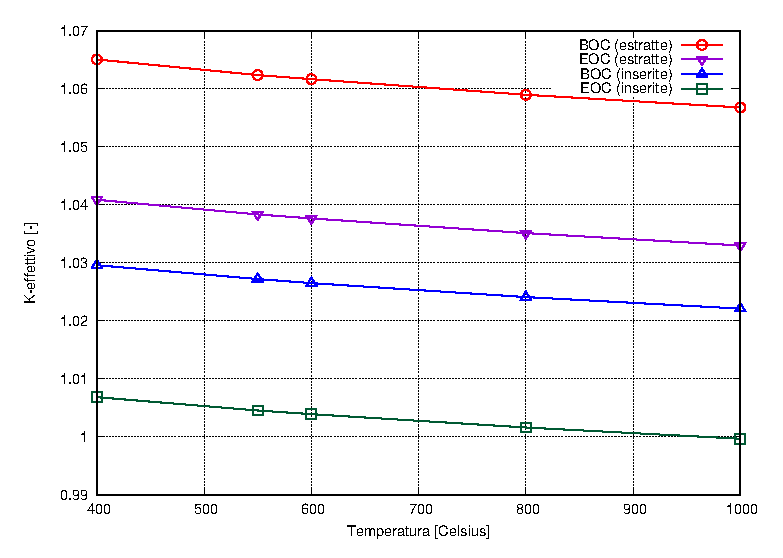
\includegraphics[scale=0.7]{../../thesis/graph/keff_temp.eps}
% % % % % % % % % %   \end{center}
% % % % % % % % % % \end{frame}
% % % % % % % % % % %%%%%%%%%%%%%%%%%%%%%%%%%%%%%%%%%%%%%%%%%%%%%%%%%%%%%%%%%%%%%%
% % % % % % % % % % %%%%%%%%%%%%%%%%%%%%%%%%%%%%%%%%%%%%%%%%%%%%%%%%%%%%%%%%%%%%%%
\begin{frame}
\frametitle{Variazioni di $k_{eff}$ in funzione dei tempi di bruciamento $t_{burnup}$}
\vspace{0.5cm}
  \begin{center}
   \includegraphics[scale=0.7]{../../thesis/graph/keff_in_out_side0-eps-converted-to}
  
  \begin{itemize}
 \item \centering Confronto tra barre inserite e estratte per temperatura 
 del combustibile $T_f$= 550 $^\circ$C e $T_f$= 1000 $^\circ$C 
\end{itemize}
\end{center}
\end{frame}
%%%%%%%%%%%%%%%%%%%%%%%%%%%%%%%%%%%%%%%%%%%%%%%%%%%%%%%%%%%%%%
%%%%%%%%%%%%%%%%%%%%%%%%%%%%%%%%%%%%%%%%%%%%%%%%%%%%%%%%%%%%%%%%%%%%%%%%%%%%%%%%
\begin{frame}
\frametitle{Distribuzione di flusso neutronico a $t_{burnup}$= 3 anni}
    \vspace{0.5cm}
 \begin{columns}
  \begin{column}{0.48\textwidth}
  \begin{center}
  \underline{Barre estratte}
  
   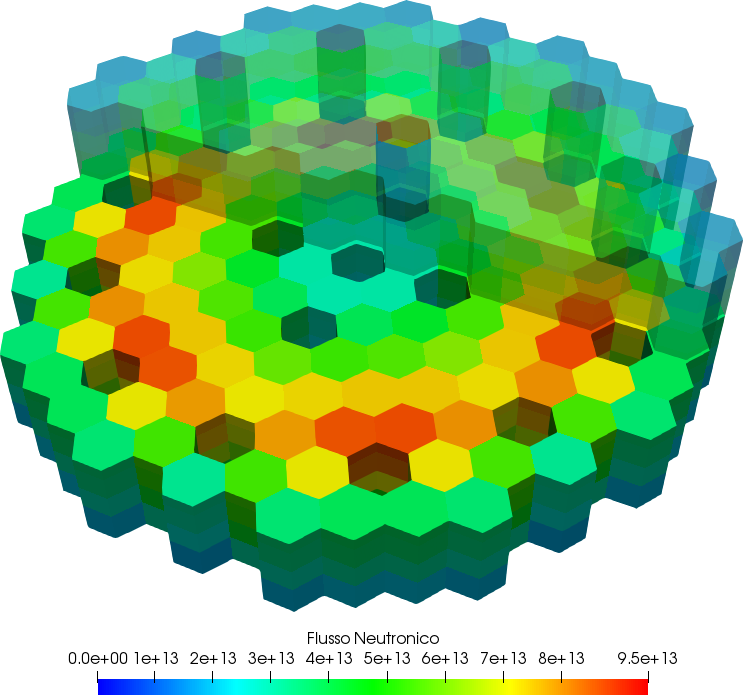
\includegraphics[scale=0.2]{../../thesis/figure/result_tred/morenew/flux-trashold-exstract1}
   
  \end{center}

  
  \end{column}

  \begin{column}{0.48\textwidth}
  
  \begin{center}
  \underline{Barre inserite}
  
   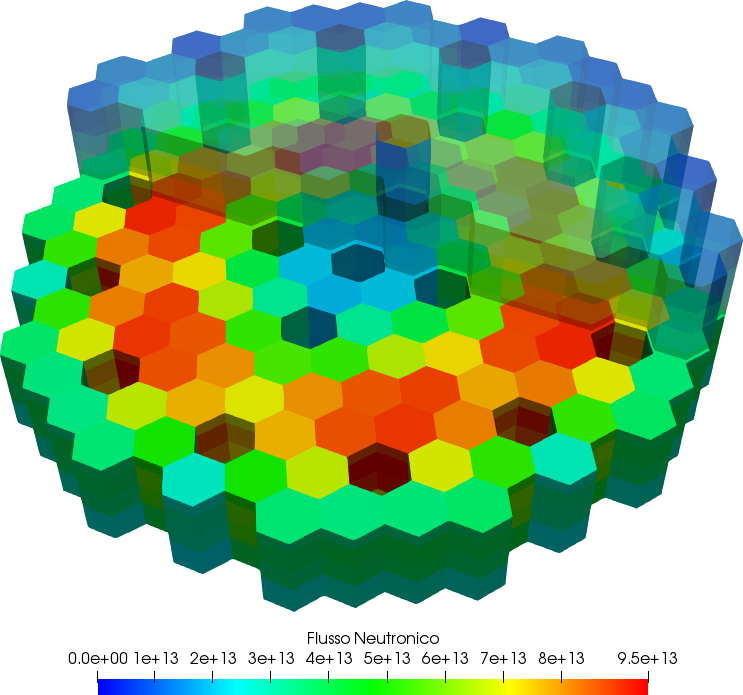
\includegraphics[scale=0.2]{../../thesis/figure/result_tred/morenew/flux-trashold-insert1}
   
  \end{center}
  
  \end{column}
  
 \end{columns}
% 
% 
\end{frame}
%%%%%%%%%%%%%%%%%%%%%%%%%%%%%%%%%%%%%%%%%%%%%%%%%%%%%%%%%%%%%%
%%%%%%%%%%%%%%%%%%%%%%%%%%%%%%%%%%%%%%%%%%%%%%%%%%%%%%%%%%%%%%%%%%%%%%%%%%%%%%%%
\begin{frame}
\frametitle{Distribuzione di potenza termica a $t_{burnup}$= 3 anni}
  \vspace{0.5cm}
 \begin{columns}
  \begin{column}{0.48\textwidth}
  
  \begin{center}
  \underline{Barre estratte}
  
   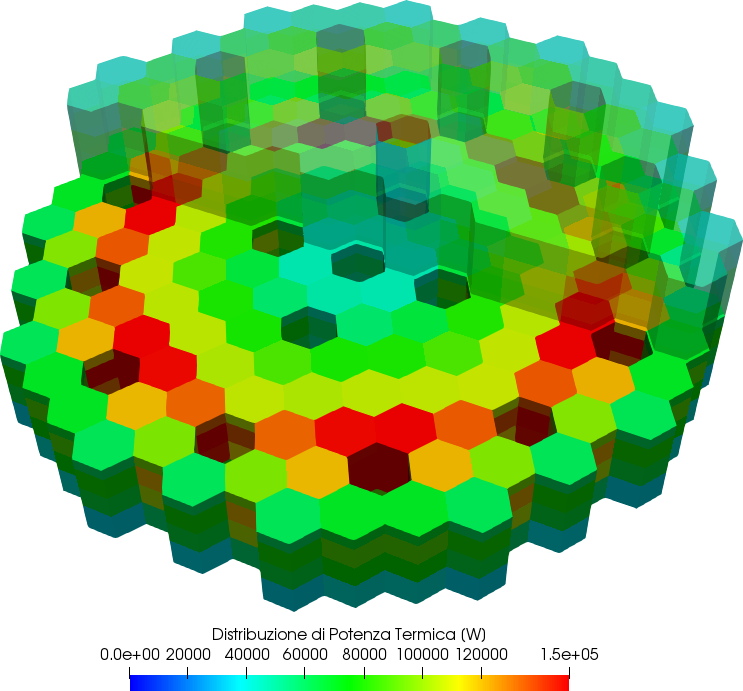
\includegraphics[scale=0.202]{../../thesis/figure/result_tred/morenew/pw-trashold-exstract1}
  \end{center}

  
  \end{column}

  \begin{column}{0.48\textwidth}
  
  \begin{center}
  \underline{Barre inserite}
  
   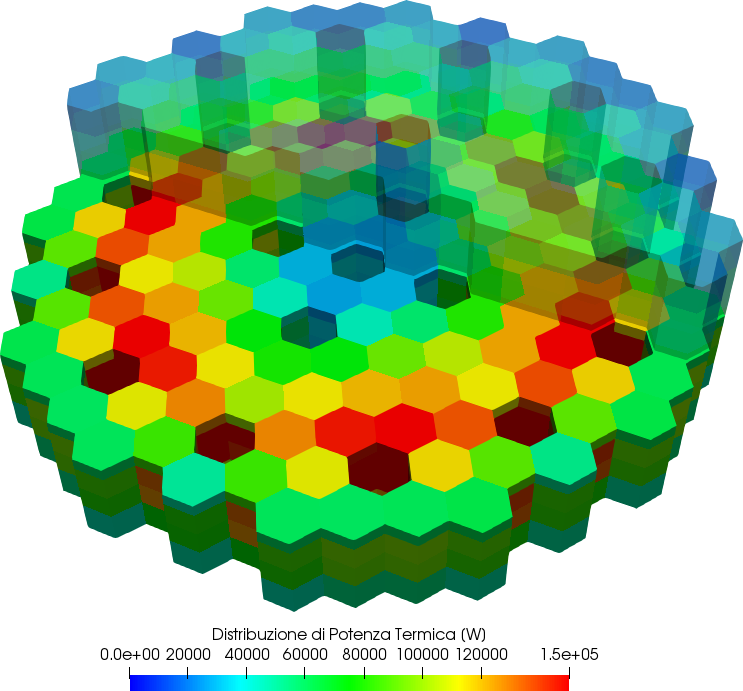
\includegraphics[scale=0.2]{../../thesis/figure/result_tred/morenew/pw-trashold-insert1}
  \end{center}
  
  \end{column}
  
 \end{columns}
% 
% 
\end{frame}
%%%%%%%%%%%%%%%%%%%%%%%%%%%%%%%%%%%%%%%%%%%%%%%%%%%%%%%%%%%%%%
% % % % %%%%%%%%%%%%%%%%%%%%%%%%%%%%%%%%%%%%%%%%%%%%%%%%%%%%%%%%%%%%%%%%%%%%%%%%%%%%%%%%
% % % % \begin{frame}
% % % % \frametitle{Confronto barre inserite e barre estratte lungo l'asse $y$}
% % % %   \vspace{0.5cm}
% % % %   
% % % %  \begin{columns}
% % % %   \begin{column}{0.48\textwidth}
% % % %   
% % % %   \begin{center}
% % % %   Distribuzione di flusso
% % % %    \includegraphics[scale=0.43]{../../thesis/graph/fluxy-eps-converted-to}
% % % %   \end{center}
% % % % 
% % % %   
% % % %   \end{column}
% % % % 
% % % %   \begin{column}{0.48\textwidth}
% % % %   
% % % %   \begin{center}
% % % %   Distribuzione di potenza termica
% % % %    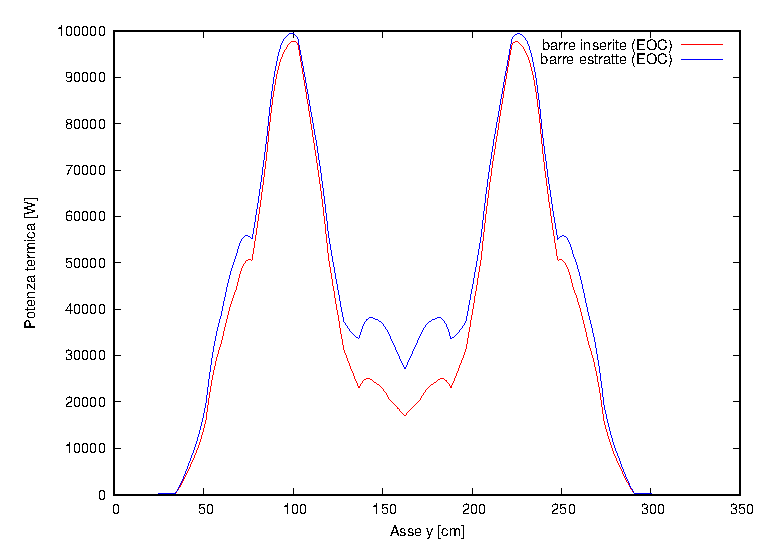
\includegraphics[scale=0.43]{../../thesis/graph/powery}
% % % %   \end{center}
% % % %   
% % % %   \end{column}
% % % %   
% % % %  \end{columns}
% % % %  \vspace{0.4cm}
% % % % %         \hspace{0.5cm}
% % % %  \begin{center}
% % % %  
% % % %  \begin{block}{Relazione tra flusso neutronico e potenza termica}
% % % % %  \hspace{1.5cm}
% % % %   \begin{equation*}
% % % %    P_{th}=E_{fissione} \cdot V_{nocciolo} \cdot \int_E \Sigma_F(E) \Phi(E)\, dE
% % % %   \end{equation*}
% % % % 
% % % %  \end{block}
% % % %   \end{center}
% % % % % 
% % % % \end{frame}
% % % % %%%%%%%%%%%%%%%%%%%%%%%%%%%%%%%%%%%%%%%%%%%%%%%%%%%%%%%%%%%%%%%%%%%%%%%%%%%%5
%%%%%%%%%%%%%%%%%%%%%%%%%%%%%%%%%%%%%%%%%%%%%%%%%%%%%%%%%%%%%%%%%%%%%%%%%%%%%%%%
\begin{frame}
\frametitle{Confronto barre inserite e barre estratte lungo un profilo radiale}
  \vspace{0.5cm}
  
 \begin{columns}
  \begin{column}{0.48\textwidth}
  
  \begin{center}
  Distribuzione di flusso
     \includegraphics[scale=0.43]{../../thesis/graph/fluxy-eps-converted-to}
%    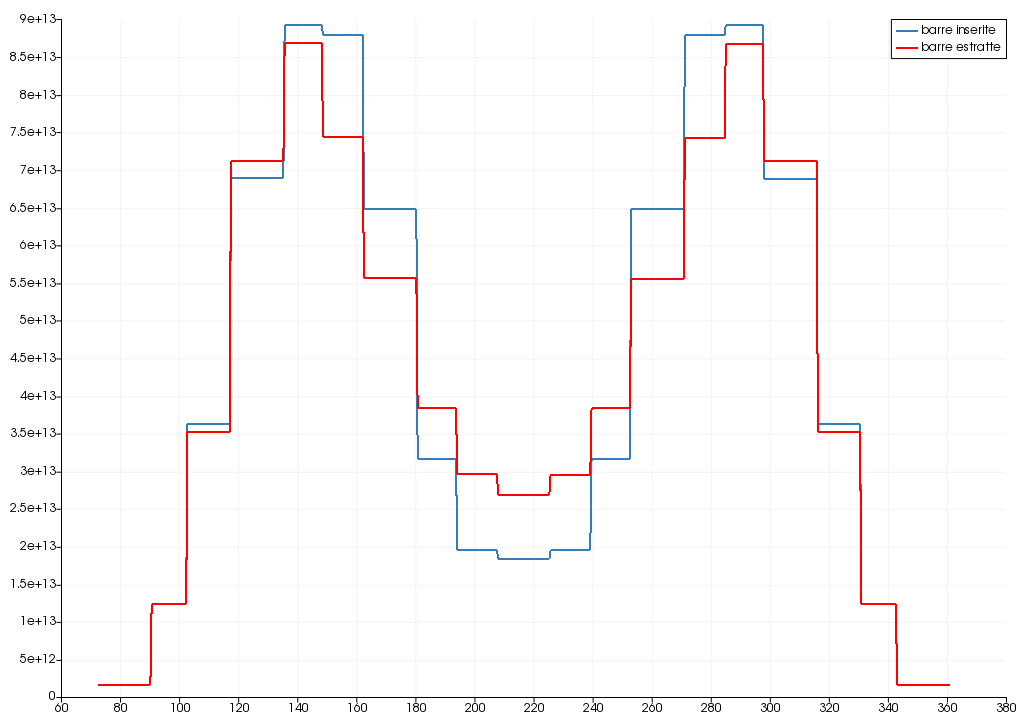
\includegraphics[height=0.38\textheight]{../flusso}
  \end{center}

  
  \end{column}
 \hspace{-1cm}
  \begin{column}{0.48\textwidth}
  
  \begin{center}
  Distribuzione di potenza termica
   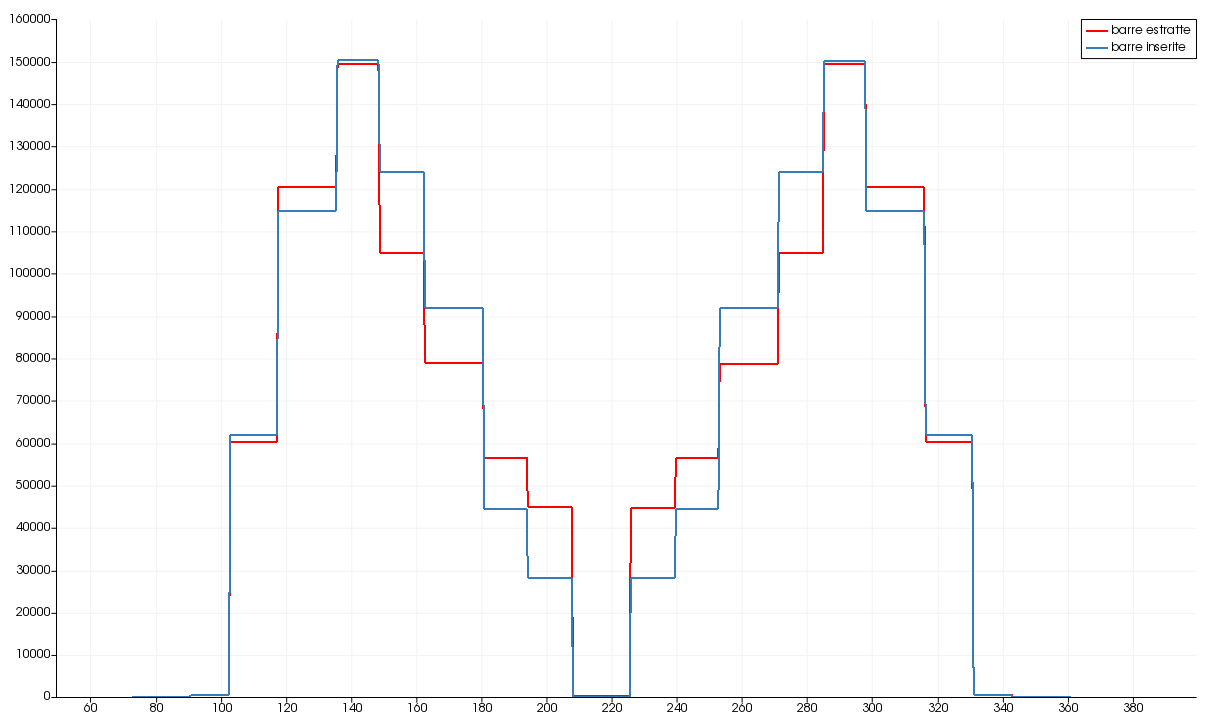
\includegraphics[scale=0.43]{../potenza}
  \end{center}
  
  \end{column}
  
 \end{columns}
 \vspace{0.4cm}
%         \hspace{0.5cm}
 \begin{center}
 
 \begin{block}{Relazione tra flusso neutronico e potenza termica}
%  \hspace{1.5cm}
  \begin{equation*}
   P_{th}=E_{fissione} \cdot V_{nocciolo} \cdot \int_E \Sigma_F(E) \Phi(E)\, dE
  \end{equation*}

 \end{block}
  \end{center}
% 
\end{frame}
%%%%%%%%%%%%%%%%%%%%%%%%%%%%%%%%%%%%%%%%%%%%%%%%%%%%%%%%%%%%%%%%%%%%%%%%%%%%%%5
\begin{frame}
\frametitle{Evoluzione del campo di temperatura}
\vspace{0.3cm} 
 \begin{columns}
  \begin{column}{0.3\textwidth}
  
  \begin{center}
  \underline{$t$= 100 secondi}
  \vspace{0.1cm}
  
   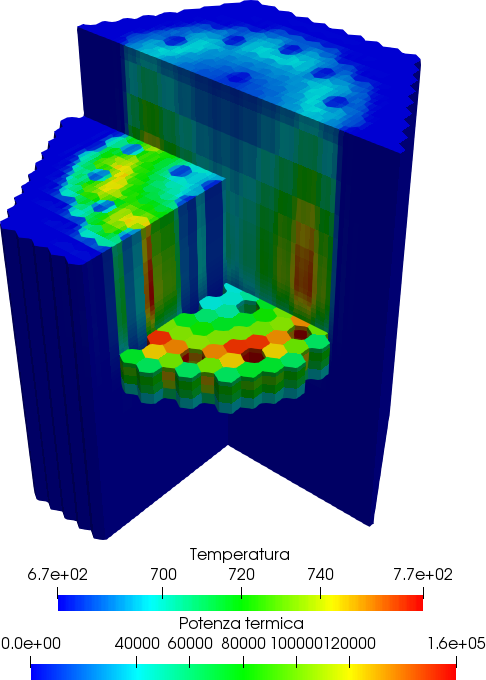
\includegraphics[scale=0.2]{../../thesis/figure/result_tred/new/tred2-temp}
   
  \end{center}

  
  \end{column}

  \begin{column}{0.3\textwidth}
  
  \begin{center}
   \underline{$t$= 250 secondi}
   \vspace{0.1cm}
   
   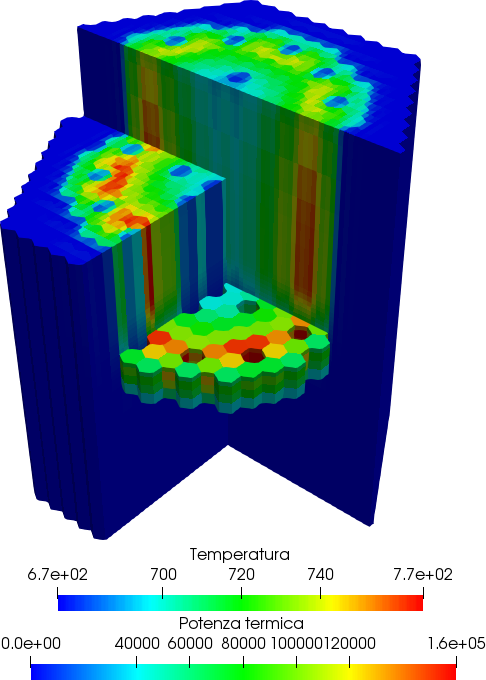
\includegraphics[scale=0.2]{../../thesis/figure/result_tred/new/tred3-temp}
  
  \end{center}
  
  \end{column}
  
   \begin{column}{0.3\textwidth}
  
  \begin{center}
   \underline{$t$= 400 secondi}
   \vspace{0.1cm}
   
   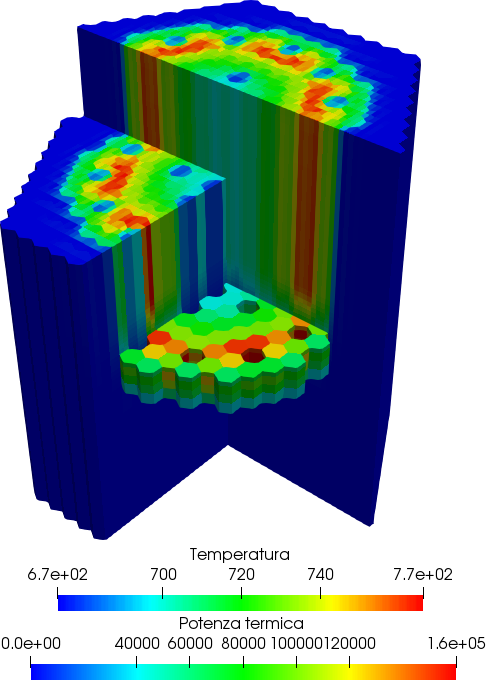
\includegraphics[scale=0.2]{../../thesis/figure/result_tred/new/tred1-temp}
  
  \end{center}
  
  \end{column}
 
 \end{columns}
 \vspace{0.3cm}
 
 \begin{center}
    Velocità del piombo liquido considerata costante \\
    \textbf{$\boldsymbol{\upsilon}$ = 1.28 m/s}
 \end{center}


% 
% 
\end{frame}
%%%%%%%%%%%%%%%%%%%%%%%%%%%%%%%%%%%%%%%%%%%%%%%%%%%%%%%%%%%%%%
%%%%%%%%%%%%%%%%%%%%%%%%%%%%%%%%%%%%%%%%%%%%%%%%%%%%%%%%%%%%%%
% % % % % % % % % % % % % % % % \begin{frame}
% % % % % % % % % % % % % % % % \frametitle{Distribuzione di temperatura lungo l'asse $z$}
% % % % % % % % % % % % % % % %   
% % % % % % % % % % % % % % % %  \begin{columns}
% % % % % % % % % % % % % % % %   \begin{column}{0.4\textwidth}
% % % % % % % % % % % % % % % %   
% % % % % % % % % % % % % % % %   \begin{center}
% % % % % % % % % % % % % % % %    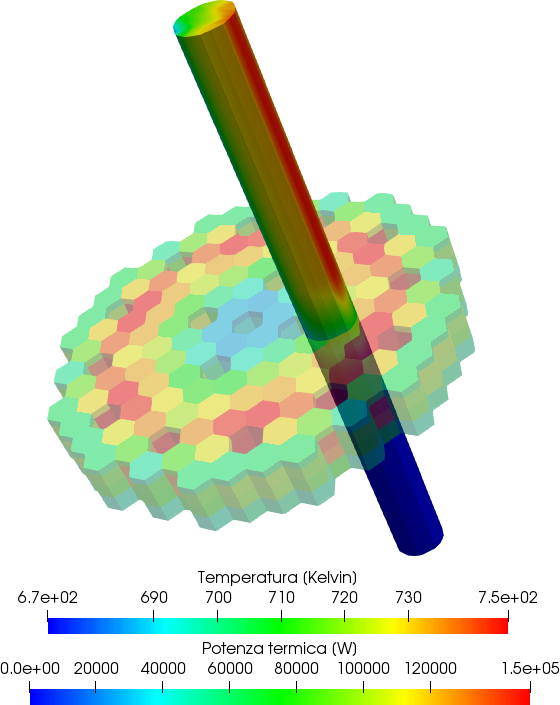
\includegraphics[scale=0.2]{../../thesis/figure/result_tred/morenew/tempassurda}
% % % % % % % % % % % % % % % %   \end{center}
% % % % % % % % % % % % % % % % 
% % % % % % % % % % % % % % % %   
% % % % % % % % % % % % % % % %   \end{column}
% % % % % % % % % % % % % % % % 
% % % % % % % % % % % % % % % %   \begin{column}{0.4\textwidth}
% % % % % % % % % % % % % % % %   
% % % % % % % % % % % % % % % %   \begin{center}
% % % % % % % % % % % % % % % %   Profilo di temperatura
% % % % % % % % % % % % % % % %    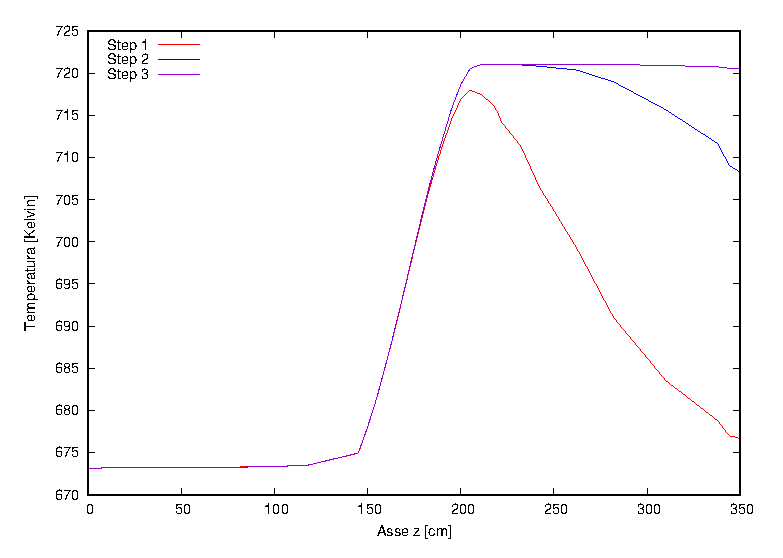
\includegraphics[scale=0.4]{../../thesis/graph/tempz}
% % % % % % % % % % % % % % % %   \end{center}
% % % % % % % % % % % % % % % %   
% % % % % % % % % % % % % % % %   \end{column}
% % % % % % % % % % % % % % % %   
% % % % % % % % % % % % % % % %  \end{columns}
% % % % % % % % % % % % % % % % % 
% % % % % % % % % % % % % % % % % 
% % % % % % % % % % % % % % % % \end{frame}
% % % % % % %%%%%%%%%%%%%%%%%%%%%%%%%%%
% % % % % % \section{Conclusioni}
% % % % % % %%%%%%%%%%%%%%%%%%%%%%%%%%%%%%%%%%%%%%%%%%%%%%%%%%%%%%%%%%%%%%%%%%%%%%%%%%%%%%%%%%%%%%%%%%%%%%%%%%%%%%%%%%
% % % % % % \begin{frame}
% % % % % % \frametitle{Conclusioni}
% % % % % % \begin{block}{Aspetti positivi}
% % % % % % \begin{itemize}
% % % % % % \item L'approccio multifisico consente di effettuare una simulazione complessiva della fisica del reattore
% % % % % % \item L'evoluzione isotopica dovuta al bruciamento è in linea con altri studi
% % % % % % \item L'accoppiamento neutronico-termoidraulico che è stato implementato apre a prospettive future per l'indagine del compormento multifisico
% % % % % % di sistemi nucleari
% % % % % % %\item La soluzione è ottenuta dopo numerose iterazione attraverso il codice di neutronica e termoidraulica con correzioni di temperatura e densità
% % % % % % %\item I risultati ottenuti aprono a prosfettivi di estendere un simile approccio ad altri modelli
% % % % % % %\item L'intera procedura è in grado di garantire flessibilità all'utente
% % % % % % \end{itemize}
% % % % % % \end{block}
% % % % % % \begin{block}{Aspetti negativi}
% % % % % % \begin{itemize}
% % % % % % \item $k_{eff}$ troppo elevato in riferimento ad altri studi del settore
% % % % % % \item Possibilità di interpolare solo su due variabili e non su tre 
% % % % % % \item Modello di termoidraulica troppo semplificativo per un'analisi approffondita
% % % % % % \end{itemize}
% % % % % % \end{block}
% % % % % % 
% % % % % % \end{frame}
% % % % % % 
% % % % % % % \section{Sviluppi Futuri}
% % % % % % \begin{frame}
% % % % % % \frametitle{Sviluppi Futuri}
% % % % % % \begin{itemize}
% % % % % % \item Aggiornamento dei dati utilizzati nella modellazione con i progetti più recenti inerenti al progetto ALFRED
% % % % % % \item Approfondimento sui sistemi di sicurezza del reattore nel codice di neutronica
% % % % % % \item Raffinazione del modello termoidraulico attraverso l'introduzione di modelli più sosfisticati e l'implementazione di codici per la turbolenza dei metalli liquidi
% % % % % % \item Estendere un simile approccio multifisico ad altri reattori
% % % % % % \end{itemize}
% % % % % % \end{frame}
% % % % % % %%%%%%%%%%%%%%%%%%%%%%%%%%%%%%%%%%%%%%%%%%%%%%%%%%%%%%%%%%%%%%%%%%%%%%%%%%%%%%%%%%%%%%%%%%%%%%%%%%%%%%%%%%


%%%%%%%%%%%%%%%%%%%%%%%%%%%
\section{Conclusioni}
%%%%%%%%%%%%%%%%%%%%%%%%%%%%%%%%%%%%%%%%%%%%%%%%%%%%%%%%%%%%%%%%%%%%%%%%%%%%%%%%%%%%%%%%%%%%%%%%%%%%%%%%%%
\begin{frame}
\vspace{0.5cm}
\frametitle{Conclusioni}
\begin{block}{Risultati Ottenuti}
\begin{itemize}
\item L'evoluzione della composizione del combustibile è in linea con altri studi
\item L'approccio multifisico consente di effettuare una simulazione complessiva della fisica del reattore
\item L'accoppiamento neutronico-termoidraulico ottenuto appare promettente e valido

% si è presentato valido, come mostrato dai risultati
%       soddisfacenti

% apre a prospettive future per l'indagine del comportamento multifisico
% di sistemi nucleari

%\item La soluzione è ottenuta dopo numerose iterazione attraverso il codice di neutronica e termoidraulica con correzioni di temperatura e densità
%\item I risultati ottenuti aprono a prosfettivi di estendere un simile approccio ad altri modelli
%\item L'intera procedura è in grado di garantire flessibilità all'utente
\end{itemize}
\end{block}
\begin{block}{Sviluppi Futuri}
\begin{itemize}
\item Aggiornamento dei dati utilizzati nella modellazione con i progetti più recenti inerenti al progetto ALFRED
\item Approfondimento sui sistemi di sicurezza (barre di controllo e di sicurezza) del reattore nel codice di neutronica
\item Raffinazione del modello termoidraulico attraverso l'introduzione di modelli più sofisticati 
      e l'implementazione di codici per la turbolenza dei metalli liquidi
% \item Estendere un simile approccio multifisico ad altri reattori
% \item $k_{eff}$ troppo elevato in riferimento ad altri studi del settore
% \item Possibilità di interpolare solo su due variabili e non su tre 
% \item Modello di termoidraulica troppo semplificativo per un'analisi approffondita
\end{itemize}
\end{block}

\end{frame}

% \section{Sviluppi Futuri}
%%%%%%%%%%%%%%%%%%%%%%%%%%%%%%%%%%%%%%%%%%%%%%%%%%%%%%%%%%%%%%%%%%%%%%%%%%%%%%%%%%%%%%%%%%%%%

\finalframe{Grazie per l'attenzione!}{../fotofancy.jpg}




\end{document}
